\section{Model případů užití (Use Case Diagram)}

\begin{figure}[H] 
  \centering
  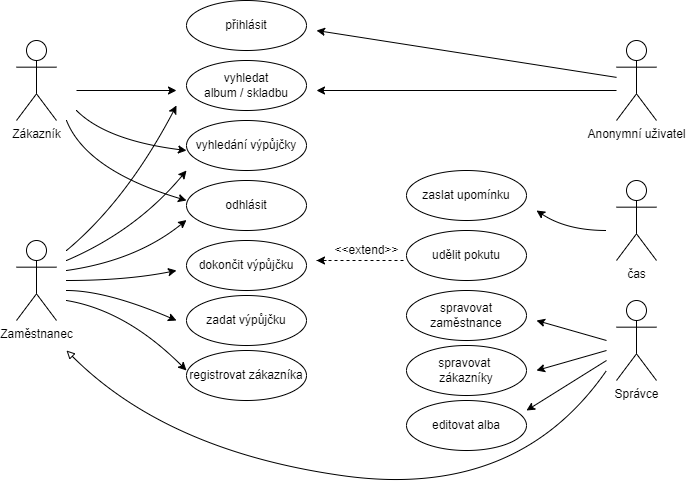
\includegraphics[scale=0.6,keepaspectratio]{usecase_diagram.png}
  \caption{Diagram připadů užití}
\end{figure}


\subsection{Popis}

\subsubsection{Anonymní uživatel}
Může vyhledat album nebo skladbu a může se přihlásit do systému.

\subsubsection{Zákazník}
Zákazník může vyhledat album nebo skladbu, vyhledat vlastní výpůjčky a podrobnosti o nich a odhlásit se ze systému.

\subsubsection{Zaměstnanec}
Zaměstnanec může vyhledat album nebo skladbu, vyhledat výpůjčky libovolného uživatele, zadat nebo dokončit výpůjčku, registrovat zákazníka a nebo se odhlásit.

\subsubsection{Správce (Zaměstnanec)}
Podle nastavených práv může správce spravovat zaměstnance, spravovat zákazníky a editovat alba.

\subsubsection{Čas}
Zasílá upomínky na vrácení výpůjčky
